\documentclass[aspectratio=43]{beamer}
\usepackage{lscape}		% Для включения альбомных страниц
\usepackage{geometry}	% Для последующего задания полей

%%% Кодировки и шрифты %%%
\usepackage{cmap}						% Улучшенный поиск русских слов в полученном pdf-файле
\usepackage[T2A]{fontenc}				% Поддержка русских букв
\usepackage[utf8]{inputenc}				% Кодировка utf8
\usepackage[english, russian]{babel}	% Языки: русский, английский
\usepackage{pscyr}						% Красивые русские шрифты

%%% Математические пакеты %%%
\usepackage{amsthm,amsfonts,amsmath,amssymb,amscd} % Математические дополнения от AMS

%%% Таблицы %%%
%\usepackage{longtable}					% Длинные таблицы
%\usepackage{multirow,makecell,array}	% Улучшенное форматирование таблиц

%%% Схемы и графики %%%
\usepackage{tikz}
\usetikzlibrary{arrows,chains,matrix,positioning,scopes,fit,shapes,decorations.markings}

%%% Общее форматирование
\usepackage[singlelinecheck=off,center]{caption}	% Многострочные подписи
%\usepackage{soul}					% Поддержка переносоустойчивых подчёркиваний и зачёркиваний

%%% Изображения %%%
\usepackage{graphicx} % Подключаем пакет работы с графикой
\graphicspath{{../Diploma/images/}} % Пути к изображениям

\usepackage{etoolbox}
\patchcmd{\theorem}{Theorem}{Теорема}{}{}
\patchcmd{\definition}{Definition}{Определение}{}{}

\usepackage{pgfpages}
%\setbeameroption{show notes on second screen}


\usetheme{Pittsburgh}
\usecolortheme{beaver}
\begin{document}
\title{Моделирование релятивистской системы квантового распределения ключей}
\subtitle{Дипломная работа}
\author{Большаков Роман Алексеевич\\ 
\textbf{Научный руководитель}: профессор,\\ д.ф-м.н. Молотков С.Н. }
\institute{Московский государственный университет имени М.В. Ломоносова\par
Факультет вычислительной математики и кибернетики\par
Кафедра суперкомпьютеров и квантовой информатики\par}
\date{Москва, 2015}
\maketitle

% \begin{frame}{Проблемы классической криптографии}
% \note{
%   В данной работе речь пойдет о квантовом распределении ключей, что является синонимом квантовой криптографии.
%   Как известно, классическая криптография делится на симметричную и асимметричную.
%   У каждой имеются свои достоинства и недостатки, однако потребоность в квантовой криптографии возникает из следующих предпосылок:
%   на слайде
% 
%   В симметричной криптографии используется один и тот же ключ как для шифрования, так и для расшифровки сообщения, что приводит к проблеме: как передать участникам передачи секретный ключ?
%   Эту проблему и решает квантовая криптография.
%   }
%   \pause
%   \begin{itemize}
%     \item проблема обнаружения подслушивателя;
%     \item основанность на предположениях об ограниченности злоумышленника в средствах, мощностях, интеллекте и др.;
%     \item асимметричная криптография требует бóльших вычислительных мощностей, чем симметричная;
%     \item абсолютная криптостойкость доказана только для шифрования по методу Вернама <<одноразовый блокнот>>;
%     \item проблема первоначальной секретности.
%   \end{itemize}
% \end{frame}

  
  \begin{frame}{Квантовая криптография}
  \note{
  Речь пойдет о квантовом распределении ключей, что является синонимом квантовой криптографии.  
 Квантовая криптография решает центральную проблему классической криптографии~--- секретное распределение ключей через открытые каналы, причем секретность гарантируется фундаментальными законами природы, что позволяет делать предположения о неограниченных вычислительных возможностях злоумышленника.}

    Квантовое распределение ключей~--- механизм:
  \begin{itemize}
    \item использующий фундаментальные принципы квантовой механики,
    \item в результате работы которого:
    \begin{itemize}
      \item либо получается \alert{общая} для двух участников коммуникации строка \alert{случайных бит}, известная \alert{только им};    
      \item либо происходит детектирование злоумышленника в канале связи.
    \end{itemize} 
  \end{itemize}
  \end{frame} 
    
  \begin{frame}
  \frametitle{Проблемы практических реализаций}
  Основные практические проблемы имеющихся на данный момент протоколов:
  \begin{itemize}
    \item лазер испускает когерентное состояние: $|\alpha\rangle = e^{-\frac{\mu}{2}} \sum_{n=0}^\infty \frac{\sqrt{\mu}}{\sqrt{n!}} |n\rangle = e^{-\frac{\mu}{2}} (|0\rangle + \sqrt{\mu}|1\rangle + \frac{\mu}{\sqrt{2}}|2\rangle + \dots)$, где $\mu$~--- среднее число фотонов в одном импульсе;
    \item потери в канале связи.
  \end{itemize}
\end{frame}
  \note{
  	Носителем \textit{ключевой} информации в идеале должны быть одиночные фотоны, но на данный момент не существует строго однофотонного источника.
  	Реально же используется сильно ослабленное лазерное излучение, которое представляет из себя суперпозицию состояний с различным числом фотонов (см формулу).
  	
  	Нестрогая однофотонность источника \textit{совместно} с потерями в канале связи приводят к ряду новых атак, например, к атаке с расщеплением по числу фотонов.
 }
 
 \begin{frame}{Атака на нерелятивистские протоколы}
   При указанных проблемах становится осуществима атака, основанная на измерениях с неопределенным исходом.
   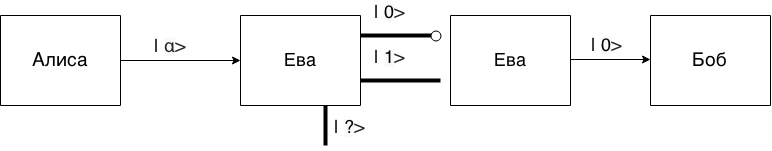
\includegraphics[width=0.9\linewidth]{um}
   \begin{center}
   	Если $Pr_{loss} > Pr_{?}$~--- подслушиватель знает весь ключ и остается незамеченным.
   \end{center}
 \end{frame}
 \note{
 	Эта атака устроена следующим образом. Ева (злоумышленник) может разорвать канал в двух местах и проводить так называемые измерения с неопределенным исходом.
 	
 	Эти измерения приводят к тому, что, начиная с некоторого уровня потерь, Ева знает ключ, не производит ошибок на приемной стороне и не детектируется.
 	}
 
 \begin{frame}{Решение проблем}
  Нерелятивистские протоколы используют \alert{только} ограничения квантовой механики.
  
  Но: \begin{itemize}
        \item фотоны движутся со скоростью света (как все безмассовые частицы),
        \item а скорость света~--- предельно допустимая скорость распространения взаимодействий.
      \end{itemize}  
  
 Квантовая механика $+$ СТО $=$ релятивистский протокол.
 \end{frame}
 \note{
 	Поэтому фундаментальных ограничений \textit{только} квантовой механики на измеримость квантовых состояний оказывается недостаточно, чтобы обеспечить секретность ключей при больших потерях.
 	 	А при передаче через открытое пространство потери достигают 5-6 порядков.
 	 	
 	 Но в открытом пространстве есть еще ограничение на движение со скоростью света, а именно~--- никакое взаимодействие не может распространяться быстрее скорости света.
 	 
 	 Поэтому в релятивистских протоколах детектируются не только ошибки, но и задержки на приемной стороне.
 }
 
 \begin{frame}{Цель дипломной работы}
   Целью данной дипломной работы является
     %\item исследовать стойкость релятивистского протокола,
     %\item исследовать количество информации, выдаваемой в ходе коррекции ошибок,
     %\item 
     создание программных средств:
   \begin{enumerate}
     \item моделирования и визуализации релятивистского протокола квантового распределения ключей в открытом пространстве,
     \item моделирования и визуализации каскадного протокола коррекции ошибок по аутентичному каналу.
   \end{enumerate}
\end{frame}
 \note{
 Целью данной дипломной работы является моделирование и визуализация такого протокола квантового распределения ключей, а также моделирование и визуализация наиболее используемого в реальных приложениях каскадного протокола коррекции ошибок.}
 
 
 \begin{frame}{Схема релятивистского протокола}
   \only<1>{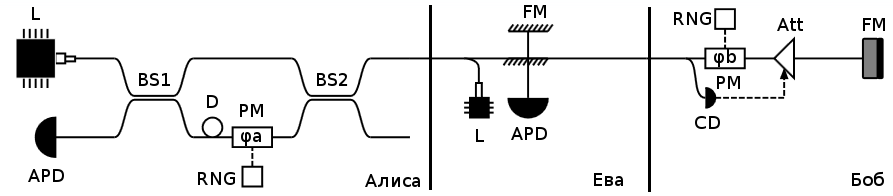
\includegraphics[width=1\linewidth]{scheme}\note{Принципиальная схема протокола показана на слайде. Суть протокола сводится к, скажем так, <<размазыванию>> информации в протяженное квантовое состояние таким образом, что по отдельности части этого состояния не несут никакой полезной информации.
 Для того, чтобы получить информацию о ключе, эти части нужно свести в одну точку пространства, на что требуется конечное время.}}
   \only<2>{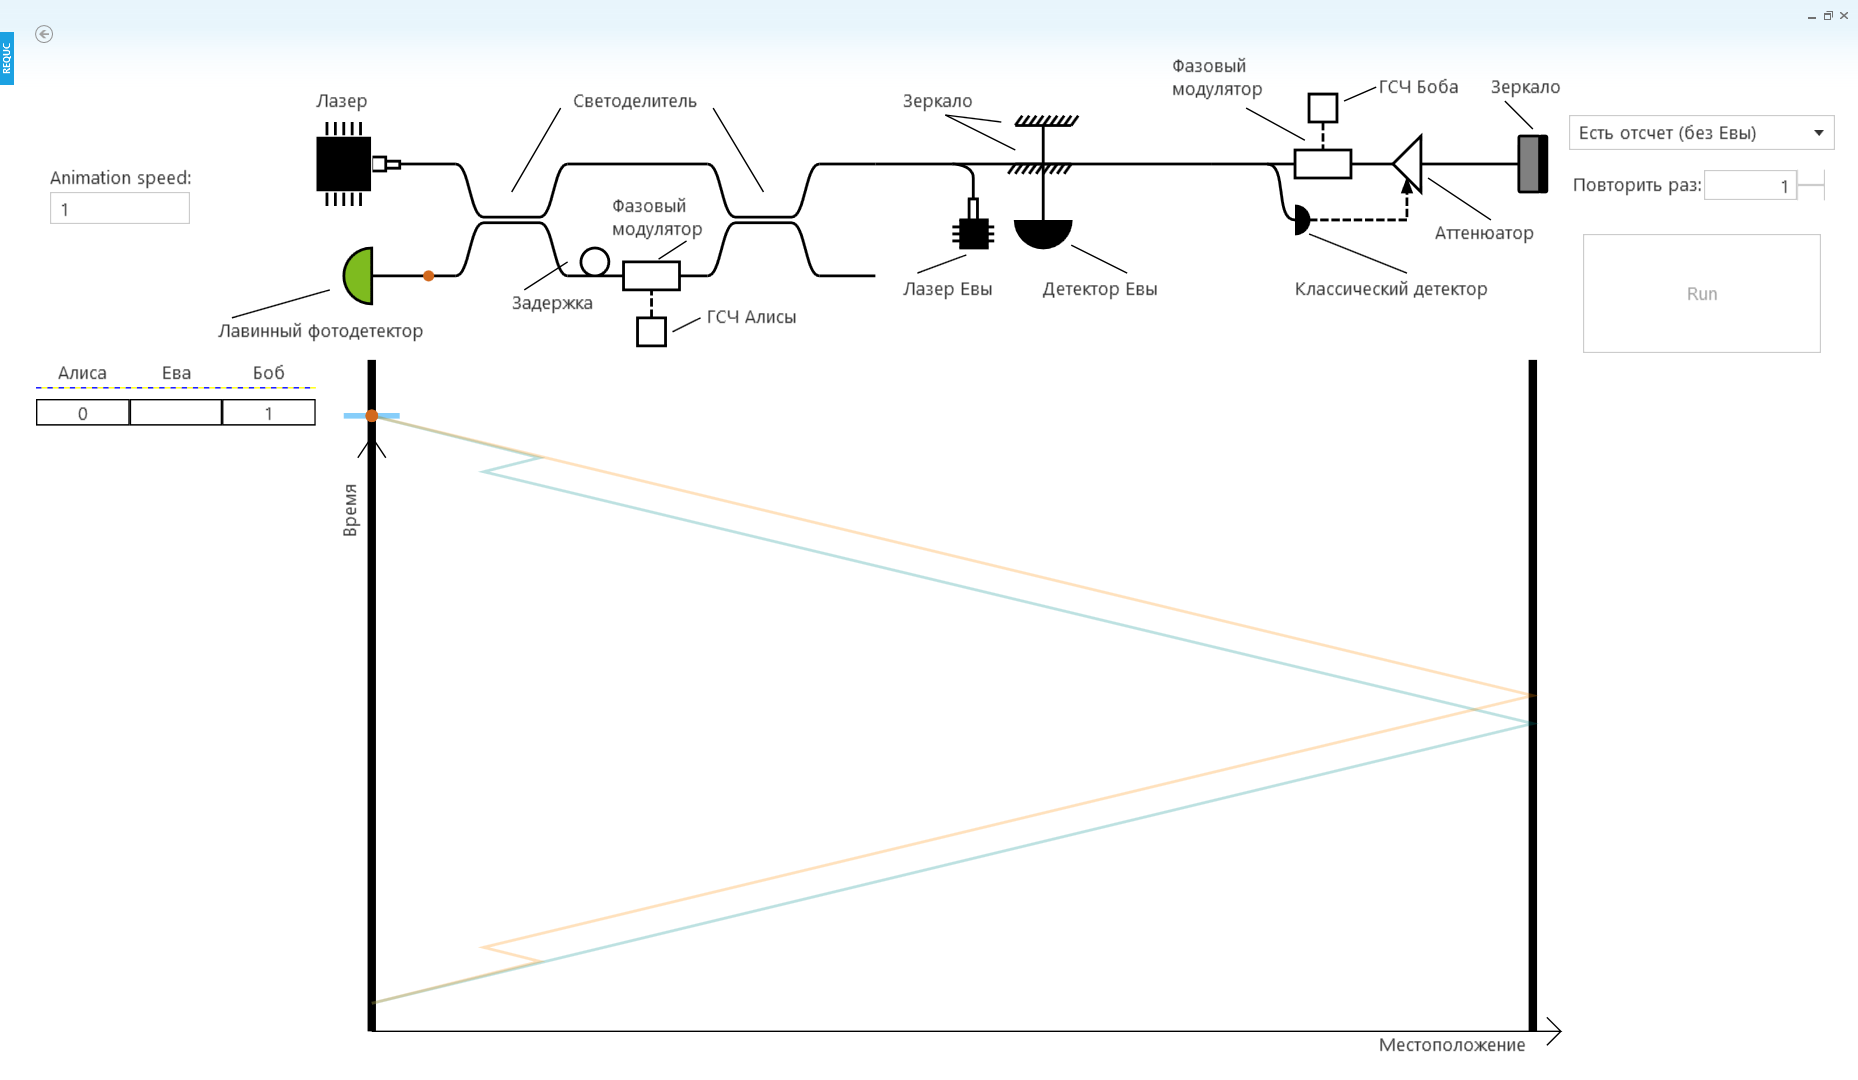
\includegraphics[width=1\linewidth]{chapter3/requc_screenshots/13_alice_detector}\note{Расстояние между участниками коммуникации всем известно и является параметром протокола. Алиса (слева) включает свой детектор только в определенные временные промежутки, когда, по ее расчетам, должно прийти ответное состояние.}}
   \only<3>{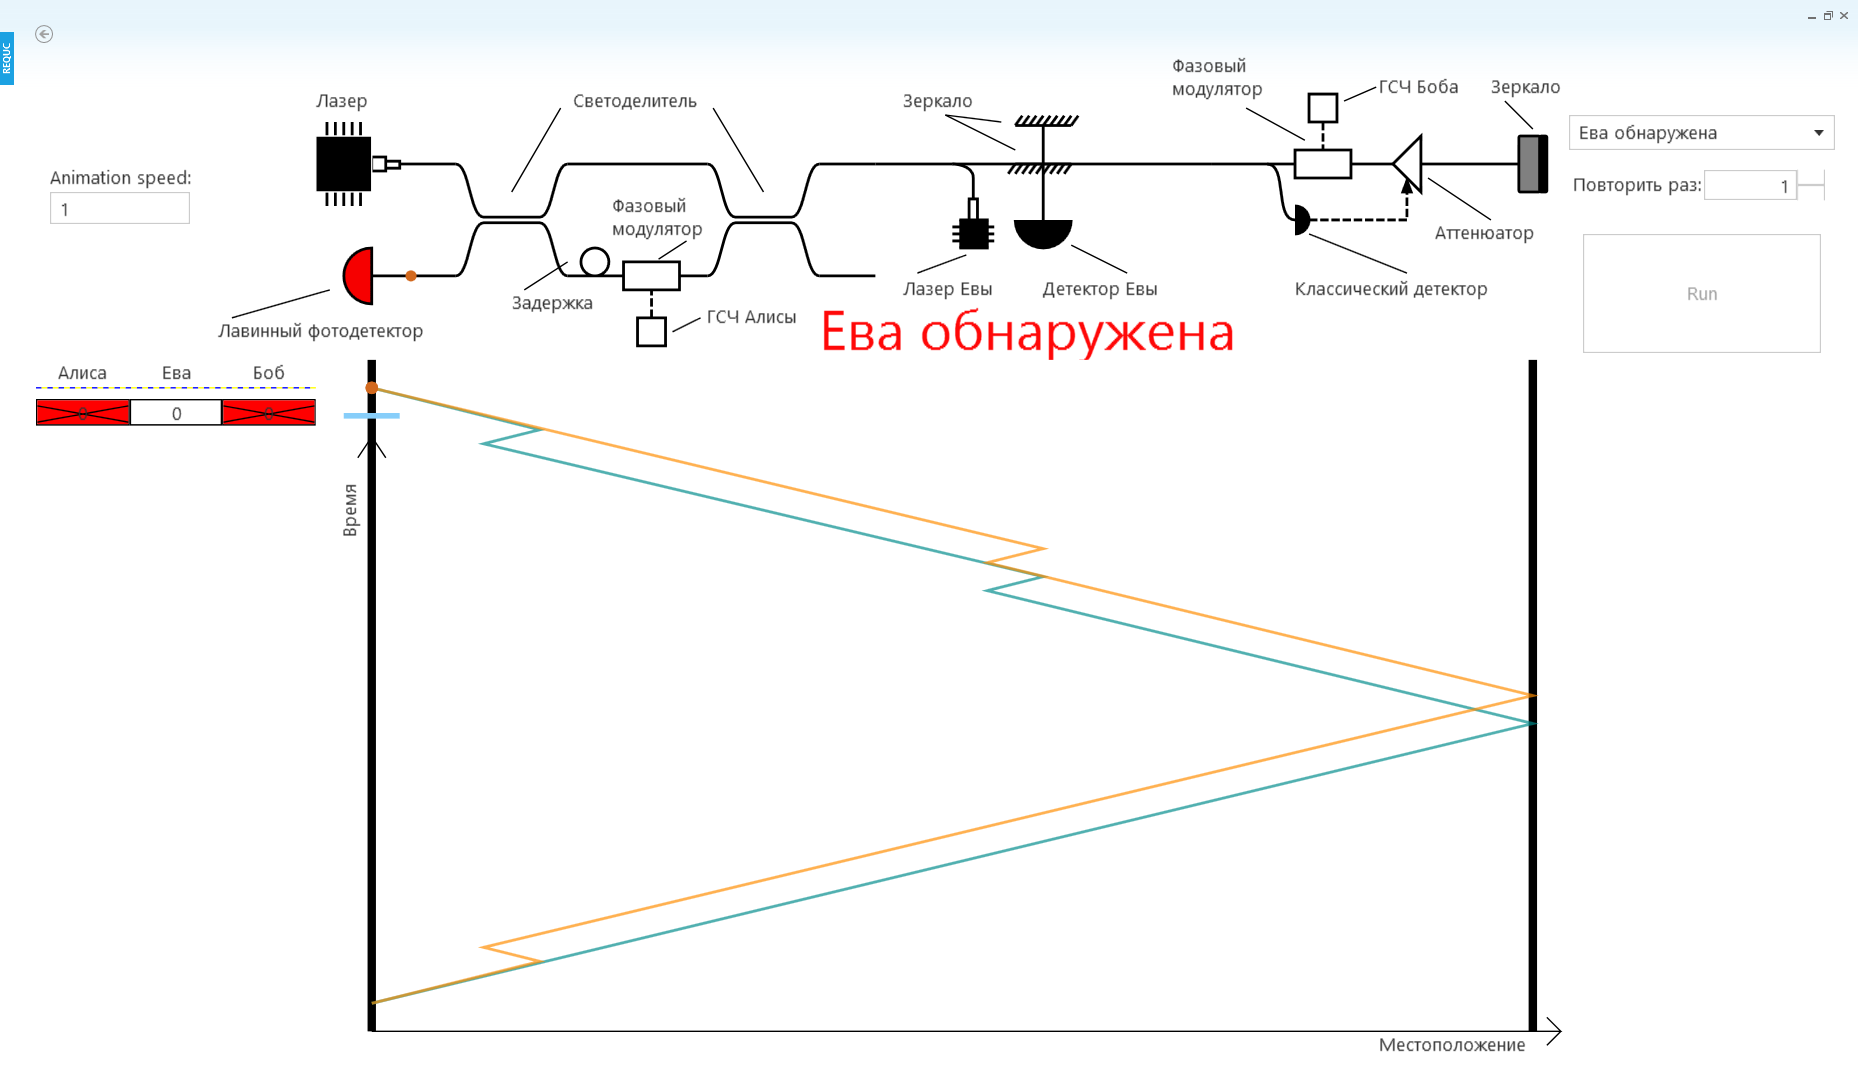
\includegraphics[width=1\linewidth]{chapter3/requc_screenshots/23_eva_detected}\note{ Если в канале передачи присутствует злоумышленник, то он потратит некоторое время сначала на сведение частей состояние вместе, получение необходимой ему информации, а затем на разведение частей обратно.
 В результате состояние придет к Алисе с задержкой, которая будет задетектирована.}}
	\only<4>{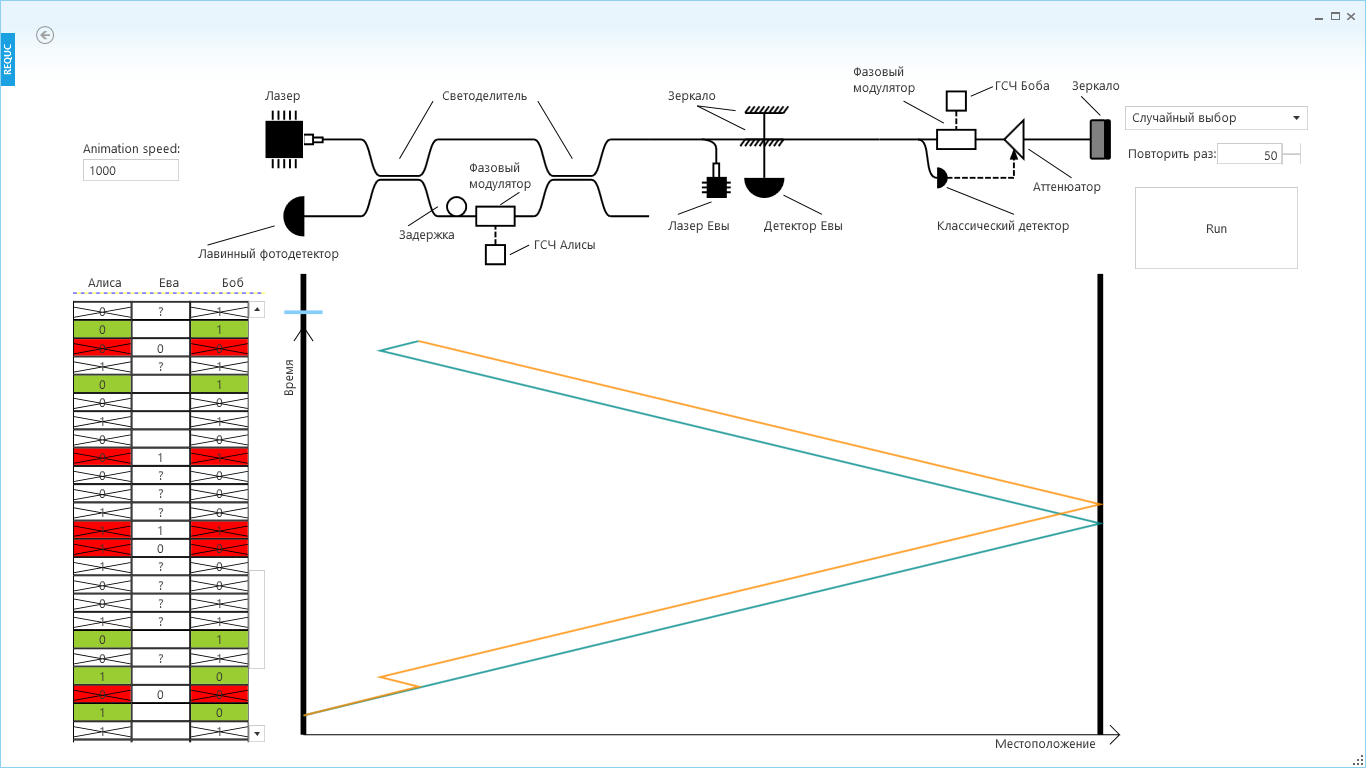
\includegraphics[width=1\linewidth]{chapter3/requc_screenshots/24_stats}\note{В результате в ключ попадет информация только из тех посылок, где Алиса получила состояние вовремя, все остальные будут отброшены}}
 \end{frame} 
  
 \begin{frame}{Каскадный метод коррекции ошибок}
     \only<1>{В канале связи (в частности если это открытое пространство) неизбежно присутствуют помехи, вносящие ошибки в ключ.
        
     Их необходимо исправить, выдав как можно меньше информации о ключе возможному подслушивателю. 
     \note{После проведения квантовой части протокола, требуется коррекция ошибок в силу наличия помех в канале связи.
 Коррекция ошибок производится по аутентичному каналу, то есть который можно свободно прослушивать, но невозможно изменить передаваемые по нему данные (газеты, twitter итд).
 После чистки ошибок требуется хэширования ключа.}}  
  \only<2>{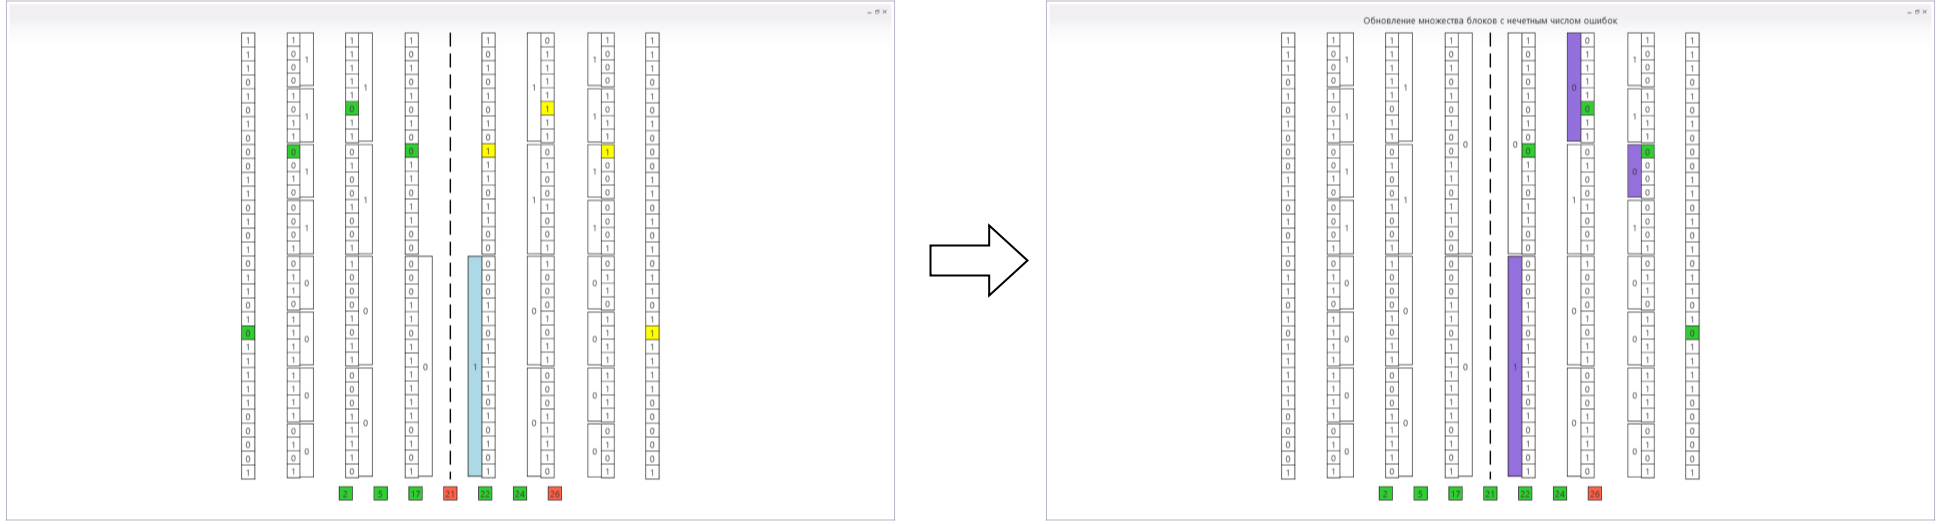
\includegraphics[width=1\linewidth]{cascade}
  	\note{Каскадный протокол коррекции ошибок является итерационной процедурой в отличие от стандартных процедур коррекции. Протокол проходит в несколько шагов, на каждом из которых исходный ключ случайным образом перемешивается, разбивается на блоки, сравниваются их четности. В блоках с несовпадающими четностями содержится как минимум одна ошибка. Каскадным он называется из-за того, что если была найдена ошибка в каком-либо блоке, то инициируется поиск ошибки во всех блоках, которые до этого содержали найденную позицию, ситуация поясняется на слайде.}}

 \end{frame}
 
 
 \begin{frame}{Сжатие полученного ключа}
 \begin{definition}
  Семейство $\mathcal{F}$ функций $\mathcal{A}\rightarrow\mathcal{B}$ называется \textit{универсальным}, если 
  $$  \pr[f(x_1) = f(x_2)] < \frac{1}{|\mathcal{B}|} ~~\forall x_1, x_2 \in \mathcal{A}: x_1 \neq x_2, $$ а $f$ выбирается из $\mathcal{F}$ в соответствии с равномерным распределением.
\end{definition}
\end{frame}
\note{После проведения процедуры коррекции ошибок Алисе и Бобу известно примерное количество информации, которое могло стать доступным Еве в ходе работы протокола распределения ключей и коррекции ошибок.
	Зная эту величину, они могут провести сжатие ключа путем хеширования функциями из универсального семейства хеш-функций, определение которого приведено на слайде. Сама хеш функция выбирается случайным образом из заранее заданного универсального семейства хеш-функций, то есть является случайной величиной.  В результате Алиса и Боб получат ключ меньшей длины, но информация Евы о нем будет бесконечно малой. 
	В итоге цель достигнута: две легитимные стороны имеют общий секретный ключ, о котором злоумышленник ничего не знает.}

 \begin{frame}{Полученные результаты}
   \begin{enumerate}
   	\item Проведен детальный анализ, моделирование и визуализация протокола квантовой криптографии, обеспечивающего безусловную секретность в условиях потерь в линии связи и неоднофотонности источника с обоснованием секретности.
	\item Рассмотрен и смоделирован (в виде отдельной программы) один из протоколов коррекции ошибок, который в настоящее время является стандартом в квантовом распределении ключей.
   \end{enumerate}
 \end{frame}
 
 \note{
 Для моделирования и визуализации релятивистского протокола квантового распределения ключей и каскадного протокола коррекции ошибок было написано две программы.
 Обе написаны на языке C\#, требуют установленного .NET 4.5, используют шаблон проектирования MVVM, и богатые возможности платформы Windows Presentation Framework (WPF) по анимации контента. 
}

\begin{frame}
	\begin{center}
		Спасибо за внимание.
	\end{center}
\end{frame}

\maketitle
\end{document}
